\documentclass[border=4pt]{standalone}
\usepackage{tikz}
\usepackage{pgfplots}
\pgfplotsset{compat=1.18}
\usetikzlibrary{shapes.geometric,arrows.meta,positioning,calc,fit,decorations.pathreplacing,backgrounds}
\definecolor{boxblue}{RGB}{225,238,252}
\definecolor{boxgreen}{RGB}{225,247,231}
\definecolor{boxorange}{RGB}{253,236,216}
\definecolor{boxgray}{RGB}{237,237,237}
\definecolor{boxred}{RGB}{253,226,226}
\begin{document}
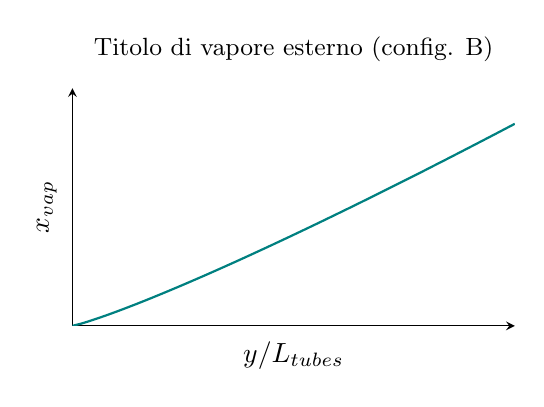
\begin{tikzpicture}
\begin{axis}[
  width=7.2cm, height=4.6cm,
  xlabel={$y/L_{tubes}$}, ylabel={$x_{vap}$},
  xtick=\empty, ytick=\empty,
  axis lines=left,
  ymin=0, ymax=1.0, xmin=0, xmax=1,
  title={\small Titolo di vapore esterno (config. B)},
]
\addplot[thick,teal,domain=0:1,samples=50]{0.85*x^1.15};
\end{axis}
\end{tikzpicture}
\hspace{0.4cm}
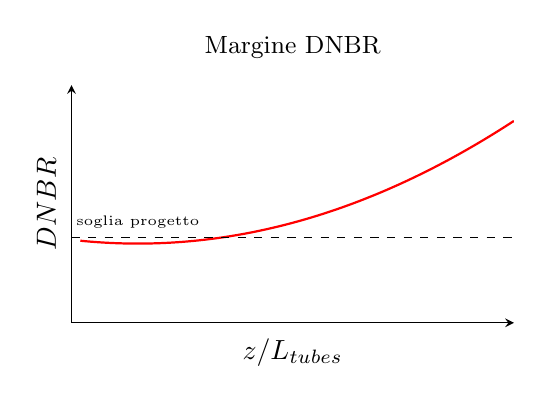
\begin{tikzpicture}
\begin{axis}[
  width=7.2cm, height=4.6cm,
  xlabel={$z/L_{tubes}$}, ylabel={$DNBR$},
  xtick=\empty, ytick=\empty,
  axis lines=left,
  ymin=0, ymax=4.2, xmin=0, xmax=1,
  title={\small Margine DNBR},
]
\addplot[thick,red,domain=0.02:1,samples=80]{1.4+3.0*(x-0.15)^2};
\draw[dashed] (axis cs:0,1.5) -- (axis cs:1,1.5) node[pos=0.15,above,font=\tiny]{soglia progetto};
\end{axis}
\end{tikzpicture}
\end{document}
